\documentclass[first=dgreen,second=purple,logo=redexc]{aaltoslides}
%\documentclass{aaltoslides} % DEFAULT
%\documentclass[first=purple,second=lgreen,logo=redque,normaltitle,nofoot]{aaltoslides} % SOME OPTION EXAMPLES

\usepackage[latin9]{inputenc}
\usepackage[T1]{fontenc}
\usepackage{graphicx}
\usepackage{amssymb,amsmath}
\usepackage{url}
\usepackage{lastpage}
\usepackage{array}
\usepackage{amsbsy}
\usepackage{multirow}
\usepackage[absolute,overlay]{textpos}
\usepackage{soul}

\newcolumntype{x}[1]{%
>{\centering\hspace{0pt}}p{#1}}%

\makeatletter
\def\thickhrulefill{\leavevmode \leaders \hrule height 1ex \hfill \kern \z@}
\def\@makechapterhead#1{%
  %\vspace*{50\p@}%
  \vspace*{11\p@}%
  {\parindent \z@ \centering \reset@font
        \thickhrulefill\quad
        \scshape \@chapapp{} \thechapter
        \quad \thickhrulefill
        \par\nobreak
        \vspace*{11\p@}%
        \interlinepenalty\@M
        \hrule
        \vspace*{11\p@}%
        \Huge \bfseries #1\par\nobreak
        \par
        \vspace*{11\p@}%
        \hrule
    %\vskip 40\p@
    \vskip 90\p@
  }}

%from here 
% fquote Fancy Quotation environment

% Use \sloppy to make right-margin easier?
% Set picture units to be relative to font size (em)?
% Use begingroup to rest units afterwards?

\newcommand{\fq@author}{}
\newcommand*{\fqsource}[1]{\gdef\fq@source{#1}}
\definecolor{quotemark}{gray}{0.7}

\newenvironment{fquote}[1][]{%
\def\fq@author{#1}% Seem to need to use def for ifx @empty to work
\let\fq@source\@empty
  \vspace{1em}
  \begin{list}{}{%
      \setlength{\leftmargin}{0.2\textwidth}
      \setlength{\rightmargin}{0.2\textwidth}
    }
    \item[]%
    \begin{picture}(0,0)(0,0)
      \put(-15,-5){\makebox(0,0){%
	  \scalebox{5}{\textcolor{quotemark}{\bfseries``}}}%
      }
    \end{picture}\em\ignorespaces%
}{%
  \newline%
  \makebox[0pt][l]{\hspace{0.6\textwidth}%
  \begin{picture}(0,0)(0,0)
    \put(15,10){\makebox(0,0){%
	\scalebox{5}{\textcolor{quotemark}{\rm\bfseries''}}}%
    }
  \end{picture}}%
  \ifx\fq@author\@empty\else\hfill\textsc{--- \fq@author}\fi
  \ifx\fq@source\@empty\else\\\mbox{}\hfill\textsl{\small\fq@source}\fi
  \end{list}
  \ifx\fq@author\@empty\else\vspace{1em}\fi
}
%to here

% Synopsis environment (like an abstract for each chapter)

\newcommand{\synopsisname}{Synopsis}

\newenvironment{synopsis}{%
%  \small
  \begin{center}%
    {\bfseries \synopsisname\vspace{-.5em}\vspace{\z@}}%
  \end{center}%
  \quotation
}{%
  \endquotation
}

\newenvironment{publish}{%
  \vfil
  \center\small\ignorespaces
  \rule{10em}{0.4pt}\par\noindent\ignorespaces
}{%
  \par\noindent\rule[1ex]{10em}{0.4pt}
  \endcenter
}


\makeatletter
% \renewcommand\bibsection%
% {
%   \section*{\refname
%     \@mkboth{\MakeUppercase{\refname}}{\MakeUppercase{\refname}}}
% }

\makeatother


\title{Mixture Models from Multiresolution 0-1 data}

\author[Prem Raj Adhikari]{ \underline{Prem Raj Adhikari}$^{1,2}$, Jaakko Hollm\'en$^{1,2}$ }
\institute[ICS]{ \hspace{0.5mm} Parsimonious Modeling Research Group in \\
$^{1}$Department of Information and Computer Science\\
\hspace{1.5mm}Aalto University School of Science, Finland\\
$^{2}$Helsinki Institute for Information Technology (HIIT) \\
%\hspace{1.5mm}Helsinki, Finland  \\
\hspace{1.5mm}\{prem.adhikari,jaakko.hollmen\}@aalto.fi \\
\hspace{1.5mm}http://users.ics.aalto.fi/padhikar/ \\
\hspace{1.5mm}Proceedings Pages: \textbf{1--16}}

\aaltofootertext{Mixture Models from Multiresolution 0--1 data} 
{Discovery Science (DS 2013), Oct. 6 to 9, 2013}
{Singapore, \insertframenumber/\inserttotalframenumber}

%\date{November 2--4, 2011}
\makeatletter

\newcommand\FrameText[1]{%
  \begin{textblock*}{0.98\textwidth}(0.2\textwidth,0.95\textheight)
    \textcolor {blue}{\scriptsize\raggedright #1\hspace{0.1\textwidth}}
  \end{textblock*}}

\begin{document}
%%%%%%%%%%%%%%%%%%%%%%%%%%%%%%%%%%%%%%%%%%%%%%%%%%%%%%%%%%%%%%%%%%%%%%%%%%%%%%%%%%%%%%%%%%%%%

\aaltotitleframe

%%%%%%%%%%%%%%%%%%%%%%%%%%%%%%%%%%%%%%%%%%%%%%%%%%%%%%%%%%%%%%%%%%%%%%%%%%%%%%%%%%%%%%%%%%%%%

% \begin{frame}
%   \frametitle{Outline}
%   \tableofcontents%[pausesections]
% 
% \end{frame}

% %%%%%%%%%%%%%%%%%%%%%%%%%%%%%%%%%%%%%%%%%%%%%%%%%%%%%%%%%%%%%%%%%%%%%%%%%%%%%%%%%%%%%%%%%%%%%
\begin{frame}{Management Summary}
\begin{itemize} \setlength{\itemsep}{6.5mm}
  \item Motivation for the Work 
  \item Multiresolution Data
  \item Mixture modelling of multiresolution data
  \item Summary and Conclusions
\end{itemize}
\end{frame}


%%%%%%%%%%%%%%%%%%%%%%%%%%%%%%%%%%%%%%%%%%%%%%%%%%%%%%%%%%%%%%%%%%%%%%%%%%%%%%%%%%%%%%%%%%%%%%%%%%%%%%

\begin{frame}
 \frametitle {Modelling : the general perspectives}
 
 \begin{fquote}[DecisionCraft Inc.]Modeling is like vintage wine; it matures with time. \fqsource{www.decisioncraft.com} \end{fquote}
 
 \pause 
 
 \begin{fquote}[Prem Raj Adhikari] People may mature with time but models mature only with increasing data. \fqsource{PhD Student} \end{fquote}


 
 \end{frame}

%%%%%%%%%%%%%%%%%%%%%%%%%%%%%%%%%%%%%%%%%%%%%%%%%%%%%%%%%%%%%%%%%%%%%%%%%%%%%%%%%%%%%%%%%%%%%%%%%%%%%%%


\begin{frame} {Importance of Using More Samples} 

\begin{alertblock}{The Square Root Law}
   $\text{Accuracy of Information} = \sqrt \text{Volume of Information}$
\end{alertblock}


 
 

\end{frame}


%%%%%%%%%%%%%%%%%%%%%%%%%%%%%%%%%%%%%%%%%%%%%%%%%%%%%%%%%%%%%%%%%%%%%%%%%%%%%%%%%%%%%%%%%%%%%%%%%%%%%%%

\begin{frame} {The Multiresolution data} 

\vspace{1mm}

\begin{figure}
\centering
  \includegraphics[trim=1cm 1cm 0.5cm 0.5cm, clip=true, width=0.8\textwidth]{figures/multires}
\end{figure}

\vspace{-3mm}

\footnotesize
$\blacksquare$ Multiresolution data is everywhere: biology, computer vision, telecoms ...

$\blacksquare$ Older Generation Technology $\Rightarrow$ Data in Coarse Resolution

$\blacksquare$ Newer Generation Technology $\Rightarrow$ Data in Fine Resolution

\end{frame}
% %%%%%%%%%%%%%%%%%%%%%%%%%%%%%%%%%%%%%%%%%%%%%%%%%%%%%%%%%%%%%%%%%%%%%%%%%%%%%%%%%%%%%%%%%%%%%%%%%%%%%%%%%%%%%%%%%%
% 
% 
% \begin{frame} {Multiresolution Data in Cancer Genomics} 
% 
% 
% \begin{figure}
% \centering
%   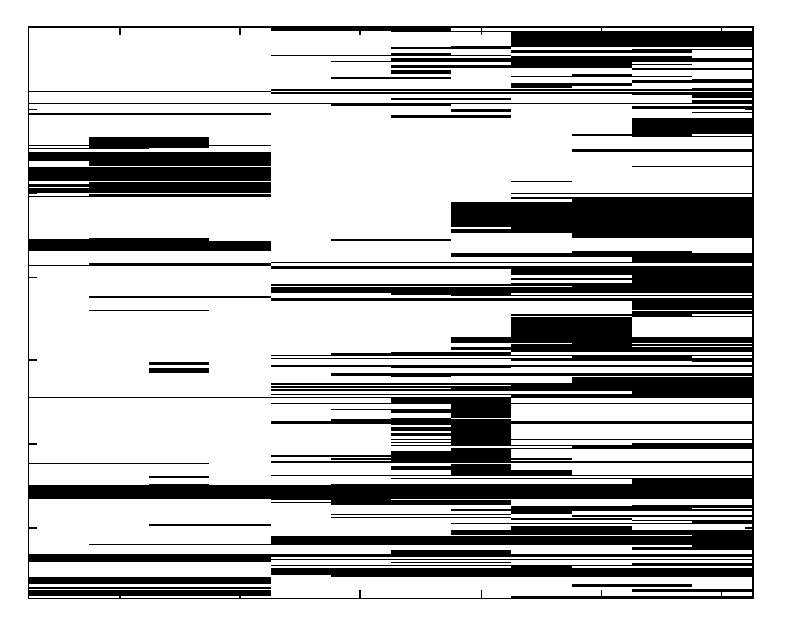
\includegraphics[width=0.8\textwidth]{figures/data}
% \end{figure}
% 
% 
% \end{frame}





%%%%%%%%%%%%%%%%%%%%%%%%%%%%%%%%%%%%%%%%%%%%%%%%%%%%%%%%%%%%%%%%%%%%%%%%%%%%%%%%%%%%%%%%%%%%%%%%%%%%%%%%%%%%%%%%%%


\begin{frame}{Chromosomal Aberrations  in Cancer}
\begin{itemize} \setlength{\itemsep}{6mm}
  \item Abnormality in the normal chromosomal content of a cell
  \item Different cases of DNA copy number aberrations
  \begin{itemize}\setlength{\itemsep}{2.5mm}
    \item Deletion: When the copy number $\boldsymbol{\textless 2} $ 
    \item Duplication: When the copy number $\boldsymbol{\textgreater 2}$
    \item Amplification: When the copy number $\boldsymbol {\gg 5}$
  \end{itemize}
  \item Why detect copy number aberrations?
  \item DNA copy number aberrations are hallmarks of cancer
  %\item {\color{red} {Why Mixture Models?}}
  %\item Cancer is a heterogeneous collection of several diseases and mixture models are well known for their 
 % ability to model heterogeneity
\end{itemize}
\end{frame}

%%%%%%%%%%%%%%%%%%%%%%%%%%%%%%%%%%%%%%%%%%%%%%%%%%%%%%%%%%%%%%%%%%%%%%%%%%%%%%%%%%%%%%%%%%%%%%%%%%%%%%%%%%%%%%%%%%%%%%%%%%%%%%%%%%%%%%5

\begin{frame}{Chromosome Nomenclature }
\begin{columns}
\column{.6\textwidth}
\begin{itemize}
  \item International System for Human Cytogenetic Nomenclature (ISCN)
  \item Short arm locations are labeled p (petit) 
  \item long arms q (queue)
  \item 17p13.2: chromosome 17, the arm p, region(band) 13, subregion(subband) 2
  \item Hierarchical, irregular naming scheme; cumbersome for scripting(manual)
\end{itemize}
\column{.4\textwidth} 
\begin{figure}
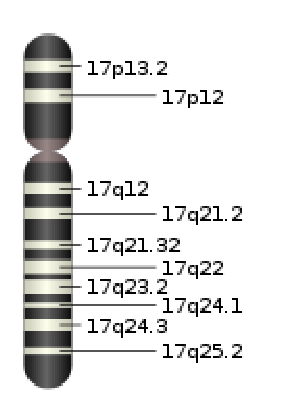
\includegraphics[height=5.7 cm]{figures/nchr17}
\end{figure}
\end{columns}
\end{frame}

%%%%%%%%%%%%%%%%%%%%%%%%%%%%%%%%%%%%%%%%%%%%%%%%%%%%%%%%%%%%%%%%%%%%%%%%%%%%%%%%%%%%%%%%%%%%%%%%%%%%%%%%%%%%%%%%%%%%%%%%%%%%%%%%%%%%%%%5

\begin{frame}{Multiple Resolutions: Chromosome-17}
\begin{figure}
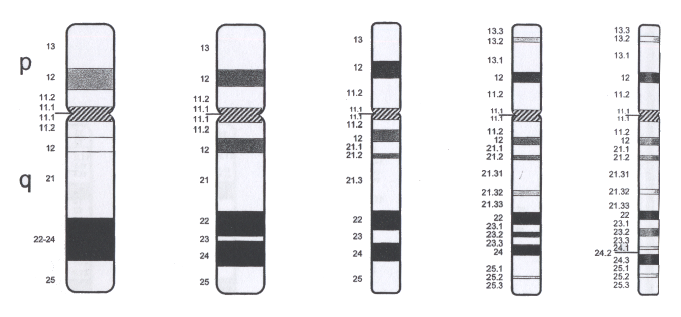
\includegraphics[width=11 cm]{figures/bands17}
\caption{G-banding patterns for normal human chromosomes at five different levels of resolution. Source: (Shaffer et. al. 2009). Example case in Chromosome:17.}
\end{figure}
\end{frame}

%%%%%%%%%%%%%%%%%%%%%%%%%%%%%%%%%%%%%%%%%%%%%%%%%%%%%%%%%%%%%%%%%%%%%%%%%%%%%%%%%%%%%%%%%%%%%%%%%%%%%%%%%%%%%%%%%

\begin{frame} {Multiresolution Data in Cancer Genomics} 

\vspace{-7mm}

\begin{figure}
\centering
  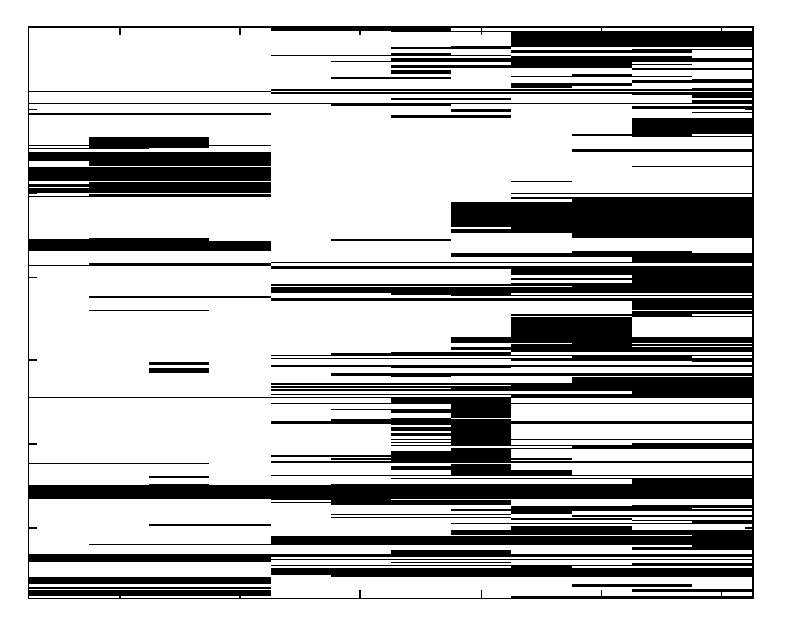
\includegraphics[width=0.7\textwidth]{figures/data}
\end{figure}

\vspace{-7mm}


\end{frame}

%%%%%%%%%%%%%%%%%%%%%%%%%%%%%%%%%%%%%%%%%%%%%%%%%%%%%%%%%%%%%%%%%%%%%%%%%%%%%%%%%%%%%%%%%%%%%%%%%%%%%%%%%%%%%%%%%%%%%%%%%%%%%%%%%%%%%%%%%%%%%%%%%%%%%%%%%%%%%%%%%%%%5

\begin{frame} {Finite Mixture Modeling 0--1 Data} 
\small
\begin{itemize}\setlength{\itemsep}{4mm}
    \item {\color{red} {Why Mixture Models?}}
    \item Cancer is a heterogeneous collection of several diseases and mixture models are well known for their ability to model heterogeneity
    
     \vspace{0.1cm}  
\textcolor{blue} { $ P(x) = \sum _{j=1}^{J} \pi _{j} P(x|\theta _{j}) = \sum _{j=1}^{J} \pi _{j} \prod _{i=1}^{d} \theta_{ji}^{x_i}(1-\theta _{ji})^{1-x_{i}}$ } \\
      \vspace{0.1cm}    
    
    \item Mixture models are probabilistic and clustering capabilities 
    \item Mixture models can be easily learned using Expectation Maximization (EM) algorithm  
    \item Open--source BernoulliMix program package to learn mixture models available from the authors \textcolor{blue}{http://users.ics.aalto.fi/jhollmen/BernoulliMix/}
\end{itemize}
\end{frame}


%%%%%%%%%%%%%%%%%%%%%%%%%%%%%%%%%%%%%%%%%%%%%%%%%%%%%%%%%%%%%%%%%%%%%%%%%%%%%%%%%%%%%%%%%%%%%%%%%%%%%%%%%%%%%%%%%%%%%%%%

\begin{frame} {Mixture Modeling of Multiresolution 0--1 Data} 
\small
\begin{itemize}\setlength{\itemsep}{4mm}
    %\item {\color{red} {Why Mixture Models?}}
    %\item Cancer is a heterogeneous collection of several diseases and mixture models are well known for their ability to model heterogeneity
    \item Mixture models generally cannot model multiresolution data
    
    \vspace{-2mm}
    
      \begin{figure}
      \centering
      \includegraphics[trim=1cm 1.3cm 1cm 1.3cm, clip=true, width=0.9\textwidth]{figures/multieq}
      \end{figure}
      
          \vspace{-2mm}

     \item Only mixture modeling solution to multiresolution data is to model each resolution separately 
     \item Multiresolution data can be transformed to single resolution for mixture modeling (Adhikari \& Hollm\'en, 2010 )
     \item Model the multiresolution data by modelling the interactions between the models in different resolutions (Adhikari \& Hollm\'en, 2012 )
\end{itemize}
\end{frame}

%%%%%%%%%%%%%%%%%%%%%%%%%%%%%%%%%%%%%%%%%%%%%%%%%%%%%%%%%%%%%%%%%%%%%%%%%%%%%%%%%%%%%%%%%%%%%%%%%%%%%%%%

% \begin{frame}{Data transformation for multiresolution modelling}
% \begin{figure}
% \centering
%   \includegraphics[trim=0cm 0cm 0cm 0cm, clip=true,width=0.60\textwidth]{figures/nweighted}
% \end{figure}
% \vspace{-5mm}
% \scriptsize
% We upsample and downsample the data and integrate the data in same resolution before mixture modelling
% \FrameText{P. R. Adhikari, J. Hollm{\'e}n, UP'2010 \\ \textbf{Patterns from Multiresolution 0-1 data}}
% \end{frame}
%%%%%%%%%%%%%%%%%%%%%%%%%%%%%%%%%%%%%%%%%%%%%%%%%%%%%%%%%%%%%%%%%%%%%%%%%%%%%%%%%%%%%%%%%%%%%

% \begin{frame}
% \frametitle{Results of Mixture Models}
% \begin{table}[h!]
%   \centering
%   \begin{tabular}{|l|c|c|}
%     \hline
%     \textbf{Data Resolution} & \textbf{J} &\textbf{Likelihood}  \\
%     \hline
%     Original in Coarse		&	8	& 	-3.39  \\ \hline
%     Original in Fine		&	8	& 	-4.75 \\ \hline
%     Downsampled to Coarse	&	6	& 	-3.41  \\ \hline
%     Upsampled to Fine		&	6	& 	-5.23  \\ \hline
%     Combined  in Coarse 	&	7	& 	-3.36  \\ \hline
%     Combined in Fine		&	7	& 	-5.11  \\ \hline     
%   \end{tabular}
%   \caption{Results of experiments on chromosome-17. J denotes the selected number of component distributions. }\label{Tab:results}
% \end{table}
% \FrameText{P. R. Adhikari, J. Hollm{\'e}n, UP'2010 \\ \vspace{-2mm} \textbf{Patterns from Multiresolution 0-1 data}}
% \end{frame}

%%%%%%%%%%%%%%%%%%%%%%%%%%%%%%%%%%%%%%%%%%%%%%%%%%%%%%%%%%%%%%%%%%%%%%%%%%%%%%%%%%%%%%%%%%%%%

% \begin{frame}{Multiresolution Mixture Modelling by Merging of Mixture Components}
% 
% \begin{itemize}
% \scriptsize \item What is done?
% \vspace{-1mm}
% \begin{figure}
% \centering
%   \includegraphics[trim=1.2cm 0cm 0cm 1cm, clip=true,width=0.72\textwidth]{figures/idasecondpage}
% \end{figure}
% \vspace{-7mm}
% \scriptsize\item How is it done?
% \scriptsize \item Fast approximation of KL divergence (P. R. Adhikari, J. Hollm\'en, DS 2012) \\ %\textcolor {red} {($\approx 10000$ times faster)}
% \scriptsize
% \textcolor{blue} {$KL  =  \displaystyle \sum_{i \in X^{*}} \pi_{\alpha} \displaystyle
% \prod _{m=1}^{{d}}
% \left(\alpha_m^{X^{*}_{im}}(1-\alpha_{m})^{(1-X^{*}_{im})} \right) -
% \displaystyle \sum_{i{\prime} \in Y^{*}} \pi_{\beta} \displaystyle \prod
% _{n=1}^{{d^{\prime}}} \left(
% \beta_{n}^{Y^{*}_{i{\prime}n}}(1-\beta_{n})^{(1-Y^{*}_{i{\prime}n})} \right)
% $}
% \scriptsize \item Retrain the mixture models in different resolutions
% \end{itemize}
% \FrameText{P. R. Adhikari, J. Hollm{\'e}n, ACML'2012 \\ \vspace{-2mm} \textbf{Multiresolution Mixture Modeling using Merging of Mixture Components}}
% \end{frame}
%%%%%%%%%%%%%%%%%%%%%%%%%%%%%%%%%%%%%%%%%%%%%%%%%%%%%%%%%%%%%%%%%%%%%%%%%%%%%%%%%%%%%%%%%%%%%
% 
% \begin{frame}{Performance of Multiresolution Mixture Model}
% \vspace{-8mm}
% \begin{figure}
% \centering
%   \includegraphics[trim=1.2cm 0cm 0cm 1cm, clip=true, width=0.97\textwidth]{figures/nbarlkhood}  
% \end{figure}
% 
% \vspace{-10mm}
% 
% \scriptsize \hspace{15mm} Better generalization through merging of mixture components
% 
% \FrameText{P. R. Adhikari, J. Hollm{\'e}n, ACML'2012 \\ \vspace{-1mm} \textbf{Multiresolution Mixture Modeling using Merging of Mixture Components}}
% \end{frame}

%%%%%%%%%%%%%%%%%%%%%%%%%%%%%%%%%%%%%%%%%%%%%%%%%%%%%%%%%%%%%%%%%%%%%%%%%%%%%%%%%%%%%%%%%%%%%%%%%%%%%%%%%%%%%%%%%%%%%%%%%%%%%

\begin{frame} {Multiresolution Mixture Components} 

      \begin{figure}
      \centering
      \includegraphics[trim=1cm 1cm 1cm 0cm, clip=true, width=0.9\textwidth]{figures/bnnfig1}
      \end{figure}
      
      \begin{itemize}\setlength{\itemsep}{2.5mm}
\item Domain ontology provides information about relationships between features in different resolutions
\item We can create a tree structure where features in the coarse resolution form the root and features in the fine resolution leaves of the tree
\end{itemize}
%\FrameText{P. R. Adhikari, J. Hollm{\'e}n, DS'2013 \\ \vspace{-2mm} \textbf{Mixture Models from Multiresolution 0-1 Data.}}
\end{frame}
%\item We can represent the tree as a Bayesian network on the assumption that the directed arrows originate from the features in the coarse resolution

%%%%%%%%%%%%%%%%%%%%%%%%%%%%%%%%%%%%%%%%%%%%%%%%%%%%%%%%%%%%%%%%%%%%%%%%%%%%%%%%%%%%%%%%%%%%%%%%%%%%%%%%%%%%%%%%%%


\begin{frame} {Bayesian Networks to Impute Missing Resolutions} 

      \begin{figure}
      \centering
      \includegraphics[trim=1cm 1cm 1cm 1cm, clip=true, width=0.9\textwidth]{figures/frobiusn}
      \end{figure}
      
      \begin{itemize}\setlength{\itemsep}{1mm}
      
      \small
\item Bayesian networks can be used to impute missing resolutions using marginal inference. 
\item For a joint distribution P(A,B,C) and an evidence B=true, marginal inference calculation is:
\hspace{5mm} $P(A\mid B=true) \propto \displaystyle\sum_C P(A,B=true,C). $


\end{itemize}

\end{frame}
%%%%%%%%%%%%%%%%%%%%%%%%%%%%%%%%%%%%%%%%%%%%%%%%%%%%%%%%%%%%%%%%%%%%%%%%%%%%%%%%%%%%%%%%%%%%%%%%%%%%%%%%%%%%%%%%%%


% \begin{frame} {Bayesian Networks to Impute Missing Resolutions} 
% 
%       \begin{figure}
%       \centering
%       \includegraphics[trim=1cm 1cm 1cm 1cm, clip=true, width=0.9\textwidth]{figures/frobiusn}
%       \end{figure}
%       
%       \begin{itemize}\setlength{\itemsep}{1mm}
%       
%       \small
% \item Bayesian networks can be used to impute missing resolutions using marginal inference. 
% \item For a joint distribution P(A,B,C) and an evidence B=true, marginal inference calculation is:
% \hspace{5mm} $P(A\mid B=true) \propto \displaystyle\sum_C P(A,B=true,C). $
% 
% 
% \end{itemize}
% \FrameText{P. R. Adhikari, J. Hollm{\'e}n, DS'2013 \\ \vspace{-2mm} \textbf{Mixture Models from Multiresolution 0-1 Data.}}
% 
% \end{frame}

%%%%%%%%%%%%%%%%%%%%%%%%%%%%%%%%%%%%%%%%%%%%%%%%%%%%%%%%%%%%%%%%%%%%%%%%%%%%%%%%%%%%%%%%%%%%%%%%%%%%%%%%%%%%%%%%%%


\begin{frame} {Structure of Mixture Model} 

      \begin{figure}
      \centering
      \includegraphics[trim=1cm 1.5cm 1cm 1cm, clip=true, width=0.9\textwidth]{figures/mixtrees}
      \end{figure}
      
      \begin{itemize}\setlength{\itemsep}{1mm}
      
\small
\item The components of the mixture model are Bayesian networks themselves 
\item Now, the problem is to learn the parameters $ \boldsymbol{\Theta}=\{J$, $\{ \pi_j,\theta_j\}_{j=1}^{J}\}$
\end{itemize}
%\FrameText{P. R. Adhikari, J. Hollm{\'e}n, DS'2013 \\ \vspace{-2mm} \textbf{Mixture Models from %Multiresolution 0-1 Data.}}

%mdlselectmultiple

\end{frame}

%%%%%%%%%%%%%%%%%%%%%%%%%%%%%%%%%%%%%%%%%%%%%%%%%%%%%%%%%%%%%%%%%%%%%%%%%%%%%%%%%%%%%%%%%%%%%%%%%%%%%%%%%%%%%%%%%%


\begin{frame} {Model Selection in Mixture Model} 

      \begin{figure}
      \centering
      \includegraphics[trim=0cm 0cm 0cm 0cm, clip=true, width=0.7\textwidth]{figures/mdlselectmultiple}
      \end{figure}
    {\footnotesize  P. R. Adhikari, J. Hollm{\'e}n, DS'2012, \textbf{Fast Progressive Training of Mixture Models for Model Selection.}}
      
   %   \begin{itemize}\setlength{\itemsep}{1mm}
      
%\FrameText{P. R. Adhikari, J. Hollm{\'e}n, DS'2013 \\ \vspace{-2mm} \textbf{Mixture Models from %Multiresolution 0-1 Data.}}

%mdlselectmultiple

\end{frame}

%%%%%%%%%%%%%%%%%%%%%%%%%%%%%%%%%%%%%%%%%%%%%%%%%%%%%%%%%%%%%%%%%%%%%%%%%%%%%%%%%%%%%%%%%%%%%%%%%%%%%%%%%%%%%%%%%%


\begin{frame} {Multiresolution Mixture Model Results} 

      \begin{figure}
      \centering
      \includegraphics[trim=1cm 0.5cm 1cm 1cm, clip=true, width=0.5\textwidth]{figures/barlkhood}
      \end{figure}
      
      \vspace{-5mm}
      
      \begin{itemize}\setlength{\itemsep}{1mm}
      
\small
\item The Y-axis shows the negative log likelihood, therefore, the shorter the bar, better the result
\item The multiresolution model outperforms single resolution models
\end{itemize}
%\FrameText{P. R. Adhikari, J. Hollm{\'e}n, DS'2013 \\ \vspace{-2mm} \textbf{Mixture Models from Multiresolution 0-1 Data.}}

\end{frame}

%%%%%%%%%%%%%%%%%%%%%%%%%%%%%%%%%%%%%%%%%%%%%%%%%%%%%%%%%%%%%%%%%%%%%%%%%%%%%%%%%%%%%%%%%%%%%%%%%%%%%%%%%%%%%%%%%%

\begin{frame}{Summary and Conclusions}

\begin{itemize} \setlength{\itemsep}{5.5mm}
 \item Mixture Modeling of Multiresolution 0--1 Data in three ways:
 \begin{itemize} \setlength{\itemsep}{4mm}
  \item Data Transformation 
  \item Merging of mixture components
  \item Bayesian network as component distributions
 \end{itemize}
 \item Experiments on multiresolution chromosomal datasets
 \item Experiments show that multiresolution models outperform single resolution models
\end{itemize}
\end{frame}


%%%% QUESTIONS FRAME BELOW %%%%%%
%%%%%%%%%%%%%%%%%%%%%%%%%%%%%%%%%%%%%%%%%%%%%%%%%%%%%%%%%%%%%%%%%%%%%%%%%%%%%%%%%%%%%%%%%%%%%



\begin{frame}
 \frametitle{Questions, Comments, Feedback and Acknowledgment}
 \begin{figure}[h!]
 \centering
 \includegraphics[width=0.5\textwidth]{figures/questions}
 \end{figure}
 
 \vspace{-15mm}
 
 \begin{figure}[h!]
 \centering
 \includegraphics[width=0.8\textwidth]{figures/logoslong}
 \end{figure}
 
 \vspace{-5mm}
 
 \small The work is funded by Helsinki Doctoral Programme in Computer Science--Advanced Computing and Intelligent Systems (Hecse)
 \end{frame}
 
%%%%%%%%%%%%%%%%%%%%%%%%%%%%%%%%%%%%%%%%%%%%%%%%%%%%%%%%%%%%%%%%%%%%%%%%%%%%%%%%%%%%%%%%%%%%%
\end{document}
